\chapter{Graph Neural Networks}

\section{Introduction}
    \begin{itemize}
        \item GNN defines a class of functions for relational reasoning over graph-structured representation.
        \item It uses \textbf{neighborhood aggregation} and \textbf{graph pooling} to solve the graph related problems
        \item Neighbor aggregation contains two important steps
        \begin{itemize}
            \item \textbf{Aggregation} - aggregating information from adjacent nodes, edges
            \item \textbf{Updation} - updating the target node with the aggregated neighborhood information.
            \item \textbf{Note}: Aggregation should be \textbf{permutation invariant operation} eg., Sum, Mean, Max
        \end{itemize}
    \end{itemize}
    
\section{GNN Pictorial Representation}
    \begin{figure}[h]
    \centering
    \begin{subfigure}[b]{0.3\textwidth}
                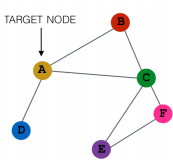
\includegraphics[width=\textwidth,height=3cm]{tex/img/Eggraph.png}
                \caption{Input Graph}
        \end{subfigure}%
        \hfill
    \begin{subfigure}[b]{0.5\textwidth}
                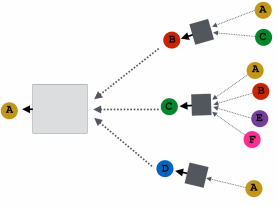
\includegraphics[width=\textwidth,height=3cm]{tex/img/GNNmodel.png}
                \caption{Neighborhood aggregation (2-layer model)}
       \end{subfigure}%
    \end{figure}

\section{Neighborhood aggregation}
    \paragraph{} Let's assume that we have only the node features and it is represented $h_{v}$ for the node $v$. Let N($v$) denotes the neighborhood of node $v$.
    \begin{equation}
        h_{v}^k = \sigma(W^k\sum_{u \in N(v)}\frac{h_u^{k-1}}{|N(v)|}+B^k h_{v}^{k-1})
    \end{equation}
    \paragraph{} The above equation represents the k-th layer of GNN with \textbf{mean aggregation} and \textbf{Neural Network updation}

\section{GNN Interpretation}
    Consider the Zachary Karate Club - a social network of a university karate club, where nodes are connected if the corresponding individuals are friends. The nodes are colored according to the different communities that exist in the network.
    \begin{figure}[h]
    \centering
    \begin{subfigure}[b]{0.5\textwidth}
                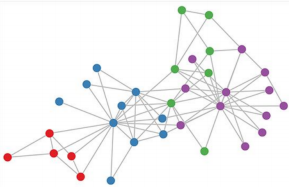
\includegraphics[width=\textwidth]{tex/img/dataset.png}
                \caption{karate club dataset}
        \end{subfigure}%
        \hfill
    \begin{subfigure}[b]{0.5\textwidth}
                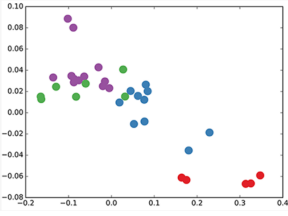
\includegraphics[width=\textwidth]{tex/img/GEmbed.png}
                \caption{Node embedding of GNN}
       \end{subfigure}%
    \end{figure}
\newpage
\section{Limitation of Neighborhood aggregation}
\paragraph{}Consider the figure below, the blue node represents the target node and it takes information from the neighbor nodes. The green and red nodes are the neighbor nodes.
\paragraph{}In mean pooling, the information gain from neighbor nodes will remain same irrespective of the dimensions. From the figure, it is shown that single dimension or two dimensions make no difference in information acquired as the no.of nodes are proportionally equal.
\paragraph{}In max pooling, the information gain remains same as the max node will be populated in the next dimension which provides the same information. So, the max or mean pooling fails.

\begin{figure}[h]
    \centering
    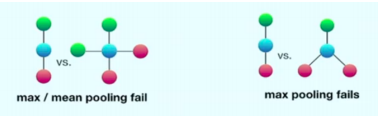
\includegraphics[width=10cm,height=3cm]{tex/img/Limitation.png}
\end{figure}